\documentclass{beamer}


\usepackage{graphicx} % Required for including images
\usepackage[utf8]{inputenc} % Required for inputting international characters
\usepackage{bookmark} % Add the bookmark package to handle changed files
\usepackage{booktabs}
\usetheme{CambridgeUS}
\usefonttheme{serif}
\usepackage{opensans}
\usepackage{amsmath}
\usepackage{amssymb}
\usepackage{amsfonts}
\usepackage{amsthm}
\usepackage{hyperref}


\usepackage{pgfplots}
\pgfplotsset{compat=1.16}
\usepackage{tikz}





\title{The Discovery of an  Algebraic structure}
\subtitle{CSMI 2024}
\author[ASSIGBE Komi. RAHOUTI Chahid.]{ASSIGBE Komi \and  RAHOUTI Chahid}
\institute[]{University of Strasbourg \\ \smallskip} 


\date[\today]{Mathematics and applications \\ \today} 
% Presentation date or conference/meeting name, 
% the optional parameter can contain a shortened version to appear on the bottom 
% of every slide, while the required parameter value is output to the title slide
%----------------------------------------------------------------------------------------
%----------------------------------------------------------------------------------------
%   TITLE SLIDE
%----------------------------------------------------------------------------------------

\begin{document}

    \begin{frame}
        \titlepage% Print the title page as the first slide
    \end{frame}
    %----------------------------------------------------------------------------------------
    %   TABLE OF CONTENTS SLIDE
    %----------------------------------------------------------------------------------------


    \begin{frame}
        \frametitle{Table of contents}
        \tableofcontents
    \end{frame}
    % ---------------------------------------------------------------------
    %   PRESENTATION BODY SLIDES
    %----------------------------------------------------------------------------------------

    \section{Introduction}
    %------------------------------------------------
    \begin{frame}
        \frametitle{Introduction}
        Many differential equations encountered 
        in solving have parametric solutions.
        Thus, to find the solution for each 
        parameter, this often requires 
        numerous calculations. To optimize 
        computation and storage times, we 
        define an algebraic structure 
        whereby, if we compute the solution 
        for parameters $\lambda_1$ and $ \lambda_2 $,
        we can deduce $\lambda_3$ ...
    \end{frame}
    %------------------------------------------------
    \begin{frame}{Example}
        Consider $u(x,\lambda)$ as a solution
        of a differential equation
        where $\lambda$ is a parameter. \\
        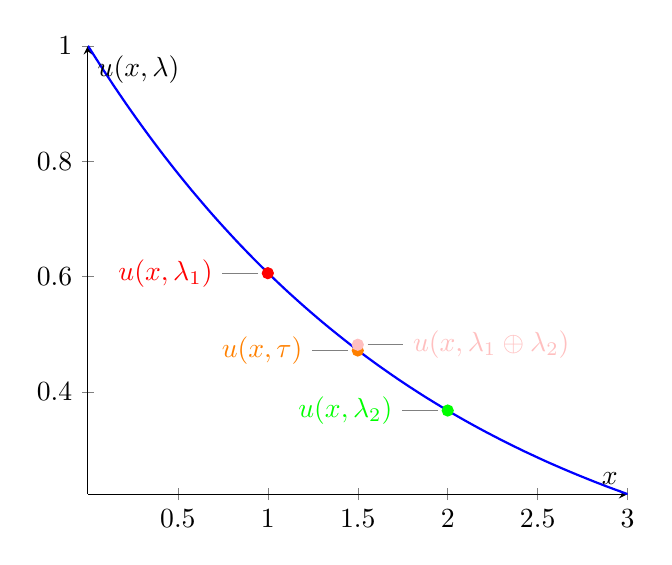
\begin{tikzpicture}
        \begin{axis}[
            axis lines = middle,
            xlabel = $x$,
            ylabel = {$u(x,\lambda)$},
            domain=0:3,
            samples=100,
            legend pos=outer north east
        ]
        \addplot[blue, thick]{exp(-0.5*x)};
        \addplot[only marks, color=red] coordinates {(1,0.606)} node[pin=180:{$u(x, \lambda_1)$}] {};
        \addplot[only marks, color=orange] coordinates {(1.5,0.472)} node[pin=180:{$u(x, \tau)$}] {};
        \addplot[only marks, color=pink] coordinates {(1.5,0.482)} node[pin=0:{$u(x, \lambda_1 \oplus \lambda_2)$}] {};
        \addplot[only marks, color=green] coordinates {(2,0.368)} node[pin=180:{$u(x, \lambda_2)$}] {};
        \end{axis}
        \end{tikzpicture}
    \end{frame}
        

        
    \begin{frame}
        \frametitle{Definition}
        What is an Algebraic structure? An algebraic structure consists of a nonempty set A (called the underlying set, carrier set or domain), a collection of operations on A (typically binary operations such as addition and multiplication), and a finite set of identities, known as axioms, that these operations must satisfy.
        Among the multiples algebraic structures, we can name:
        \begin{itemize}
            \item Group
            \item Ring
            \item Field
            \item Vector space
            \item .....
        \end{itemize}
    \end{frame}
    %------------------------------------------------

    %---------------------------------------------------------------------------------
    \section{Objectives}
    \begin{frame}
        \frametitle{Objective}
        Our Main objective consist,  if we are giving a set of data in V, and those data is defined on a regular surface and we want to know if it is possible to detect a certain algebraic structure using Neural Networks Learning.
    \end{frame}


    \subsection{First sub objective} 
    \begin{frame}
        \frametitle{Identify The Best Approch}
        The Best way that we choose to attack the problem  is to consider a function $f$ that can map the binary operations defined on $V$ to a binary operation defined on $\mathbb{R}$ that satisfy this theorem : 
        \begin{theorem}\label{thm:1}
            \rm{
            Let $\mathbb{R}$ be the field of real numbers and let $f: \mathbb{R} \rightarrow V$ be a one-to-one function from $\mathbb{R}$ onto a codomain $V$. If we define vector addition by
            $$
            x \oplus y=f\left(f^{-1}(x)+f^{-1}(y)\right)
            $$
            and scalar multiplication by
            $$
            \alpha \odot x=f\left(\alpha \cdot f^{-1}(x)\right)
            $$
            for all $x$ and $y$ in $V$ and all $\alpha$ in $\mathbb{R}$, then 
            $(V, \oplus, \odot)$. is a vector space over $\mathbb{R}$.
            }
        \end{theorem}
    \end{frame}
    
    \begin{frame}
        \frametitle{Example}
        \begin{itemize}
            \item Let $\beta$ be any positive real number and let $f: \mathbb{R} \rightarrow \mathbb{R}^{+}$be defined by $f(x)=(1 / \beta) e^x$. Then $f$ is a one-to-one function from $\mathbb{R}$ onto the set of positive real numbers, and $f^{-1}(x)=\ln (\beta x)$ for $x>0$. we would define vector addition and scalar multiplication by
            $$ 
            x \oplus y=\frac{1}{\beta} e^{\ln (\beta x)+\ln (\beta y)}=\beta x y
            $$
            $$
            \alpha \odot x=\frac{1}{\beta} e^{\alpha \ln (\beta x)}=\beta^{\alpha-1} x^\alpha.
            $$
            \end{itemize}
    \end{frame}
    %---------------------------------------------------------------------------------
    \begin{frame}
        As we see this theorem based if we have a function
        $f$ one-to-one and verify the two proprieties we can conclude that the dataset V is a vector space.
        So, the challenge for us if we are given a set of points $V$ is it  possible to 
        find $(\oplus,\odot,f,f^{-1})$ that satisfy the conditions of the theorem ?
    \end{frame}





    \subsection{Second sub objective}
    \begin{frame}

        \frametitle{Implementing the 2D case}


        We will consider this dataset 
        $(\mathbf{x}, \mathbf{x}+\varepsilon \sin (\mathbf{x} / \varepsilon))$ with $\varepsilon \rightarrow 0$.
        \\
        Then we will try to find the best function $f$ that can map the binary operations defined on $V$ to a binary operation defined on $\mathbb{R}$  the theorem \ref{thm:1}.
        \newpage
        \begin{figure}
            \centering
            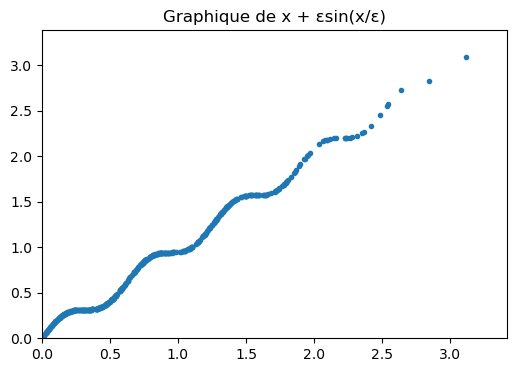
\includegraphics[width=0.5\textwidth]{./images/M.png}
            \caption{$(\mathbf{x}, \mathbf{x}+\varepsilon \sin (\mathbf{x} / \varepsilon))$,  $\varepsilon = 0.1$, with 2000 points, $x$ following a uniform distribution}
            \label{fig:1}
        \end{figure}
        
    \end{frame}
    %---------------------------------------------------------------------------------
    \section{Mathematical setting}
    \begin{frame}
        \frametitle{Mathematical setting}
        In use of the theorem \ref{thm:1}, we can define the following loss function in order to find the best  quadruplet ${\theta}(\oplus,\odot,f,f^{-1})$ that can map the binary operations defined on $V$ to a binary operation defined on $\mathbb{R}$.


        \begin{enumerate}
            \item Loss for vector addition:
            \[
                L_1(\theta) = \sum_{(x, y) \in V \times V} \left\lVert x \oplus y - f(f^{-1}(x) + f^{-1}(y))\right\rVert_{V}^2
            \]
            \item Loss for scalar multiplication:
            \[
                L_2(\theta) = \sum_{(\alpha, x) \in \mathbb{R} \times V} \left\lVert \alpha \odot x - f(\alpha \cdot f^{-1}(x)) \right\rVert_{V}^2
            \]
        \end{enumerate}
    
        Function $L(\theta)$, the sum of these two functions:
        \[
        L(\theta) = L_1(\theta) + L_2(\theta)
        \]
    
        We  precise that the norm $\left\lVert \cdot \right\rVert_{V}$ is the norm defined on the dataset $V$.
    \end{frame}
    %---------------------------------------------------------------------------------


    
    \section{Tools}
    \begin{frame}{Tools}
        For the implementation of this project, we use :
        \begin{itemize}
            \item Python, Pytorch Library 
            \item Neural Networks learning by transforming the axioms of
            an Algebraic structure into a loss to minimize.
            \item slack to communicate and share Idea
            \item Git to share code and work together
        \end{itemize}
    \end{frame}
    
    \section{Numerical Experiments}
    \begin{frame}{}
        \frametitle{The Training Data}
        In order to test the efficiency of our approach, we will consider the following dataset:
        $(\mathbf{x}, \mathbf{x}+\varepsilon \sin (\mathbf{x} / \varepsilon))$.
            \\
            The parameters used for the training are:
            \begin{itemize}
                \item $\mathbf{x}$ is randomly generated from a uniform distribution.
                \item $\varepsilon = 0.1$
                \item  $dim_E = 2$ like the dataset is defined on a 2D,
                the abscissa and the ordinate.
                \item The Number of Epochs = 1000  to train the model.
                \item The learning rate = 1e-3
                \item The Number of Points = 2000
            \end{itemize}

            The Training Dataset is shown in Figure~\ref{fig:1}.
    \end{frame}
    %---------------------------------------------------------------------------------
    \begin{frame}
        \frametitle{The result of the training}
        The evolution of the loss function during the training : 
        \begin{table}[h]
            \centering
            \begin{tabular}{|c|c|c|c|}
            \hline
            Epoch & $L_{1}$ & $L_{2}$ & $L = L_{1} + L_{2}$ \\
            \hline
            0/1000 & 79.302979 & 96.402763 & 175.705750 \\
            200/1000 & 8.830682 & 12.671237 & 21.501919 \\
            400/1000 & 0.064797 & 0.174934 & 0.239731 \\
            600/1000 & 0.021591 & 0.010077 & 0.031668 \\
            800/1000 & 0.017061 & 0.011970 & 0.029031 \\
            \hline
            \end{tabular}
            \caption{Training results with 64 neurons per layer for the Loss}
        \end{table}
    \end{frame}

    \begin{frame}
        The representation of the loss function during the training : 
        \begin{figure}[h]
            \centering
            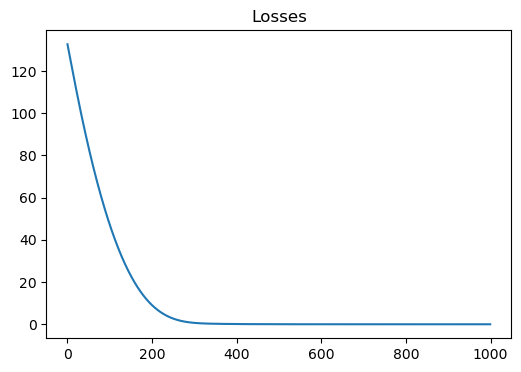
\includegraphics[width=0.8\textwidth]{./images/losses.png}
            \caption{Losses during training}
            \label{fig:losses}
        \end{figure}
    \end{frame}

    \section{Test}
    \begin{frame}
        \frametitle{Test Data}
        To test the efficiency of our approach, we will consider the following points belonging to the dataset which are unknown to the model, following a normal distribution:
        \begin{table}[h]
            \centering
            \begin{tabular}{|c|c|c|c|c|}
                \hline
                B\_x & B\_y & C\_x & C\_y & $\alpha$ \\
                \hline
                0.133921 & 0.231251 & -0.364604 & -0.316272 & 0.131015 \\
                -0.135106 & -0.232701 & -0.183459 & -0.280000 & 0.632417 \\
                -0.075604 & -0.144208 & 0.518957 & 0.430128 & -0.094283 \\
                -0.272498 & -0.312965 & -0.355346 & -0.315314 & 1.490005 \\
                -0.053795 & -0.105033 & 0.319357 & 0.314162 & -0.585686 \\
                0.038281 & 0.075634 & 0.252877 & 0.310395 & 0.982973 \\
                0.517463 & 0.427957 & -0.361297 & -0.315886 & -1.826494 \\
                -0.249884 & -0.309824 & 0.505564 & 0.411397 & -1.387667 \\
                0.166805 & 0.266332 & 0.296044 & 0.314060 & -1.156715 \\
                0.345609 & 0.314675 & -0.408402 & -0.327503 & -0.028152 \\
                \hline
            \end{tabular}
            \caption{Points belonging to the dataset}
        \end{table}
    \end{frame}

    \subsection{First Property of theorem}
    \begin{frame}
        \frametitle{First Property of theorem}
        After we apply the model to the test data, we obtain the following results:
        \begin{center}
            \resizebox{\textwidth}{!}{%
                \begin{tabular}{|c|c|c|c|c|}
                \hline
                $(x_i, y_i)$ & $f_{\theta}(f_{\theta}^{-1}(B) + f_{\theta}^{-1}(C))$ & $B\oplus_{\theta} C$ & $Erreur L^2$ & $Erreur  inf$ \\
                \hline
                $(x_1, y_1)$ & $(0.025816463, -0.064952835)$ & $(0.027578719, -0.06542145)$ & $1.8e-03$ & $1.5e-03$ \\
                $(x_2, y_2)$ & $(0.025946498, -0.06484896)$ & $(0.025081158, -0.068941236)$ & $4.2e-03$ & $2.7e-03$ \\
                $(x_3, y_3)$ & $(0.019929841, -0.070546366)$ & $(0.019148044, -0.07449238)$ & $4.0e-03$ & $3.8e-03$ \\
                $(x_4, y_4)$ & $(0.028739408, -0.062192287)$ & $(0.029816508, -0.06403735)$ & $2.1e-03$ & $1.3e-03$ \\
                $(x_5, y_5)$ & $(0.021517947, -0.06903623)$ & $(0.021849744, -0.07182622)$ & $2.8e-03$ & $1.6e-03$ \\
                $(x_6, y_6)$ & $(0.021567993, -0.068980195)$ & $(0.023057297, -0.07014613)$ & $1.9e-03$ & $1.5e-03$ \\
                $(x_7, y_7)$ & $(0.02241145, -0.06818917)$ & $(0.023231708, -0.07093868)$ & $2.9e-03$ & $2.7e-03$ \\
                $(x_8, y_8)$ & $(0.021432638, -0.06912259)$ & $(0.020650879, -0.072933406)$ & $3.9e-03$ & $3.8e-03$ \\
                $(x_9, y_9)$ & $(0.02023638, -0.070240326)$ & $(0.02151636, -0.071243554)$ & $1.6e-03$ & $1.3e-03$ \\
                $(x_{10}, y_{10})$ & $(0.024316281, -0.06637937)$ & $(0.02585955, -0.067992836)$ & $2.2e-03$ & $1.6e-03$ \\
                \hline
                \end{tabular}%
            }
            \end{center}
            \end{frame}
            \begin{frame}
                \begin{columns}
                    \begin{column}{0.5\textwidth}
                        \centering
                        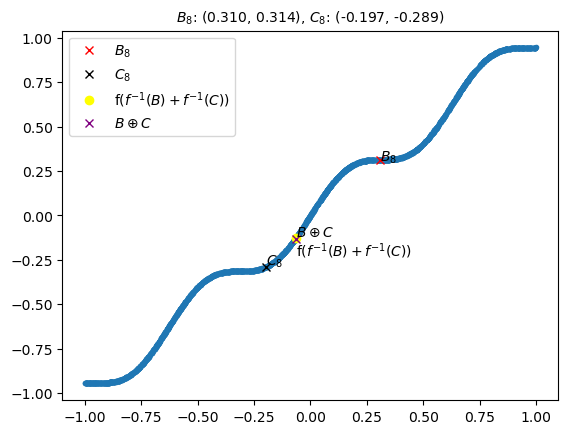
\includegraphics[width=0.9\linewidth]{./images/1.png}
                    \end{column}%
                    \begin{column}{0.5\textwidth}
                        \centering
                        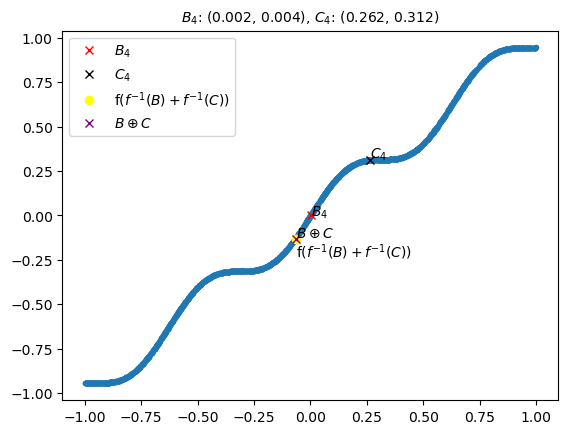
\includegraphics[width=0.9\linewidth]{./images/2.png}
                    \end{column}
                \end{columns}
            \end{frame}
            %---------------------------------------------------------------------------------
            \subsection{Second Property of theorem}
            \begin{frame}
                \frametitle{Second Property of theorem}
                Doing the same thing for the scalar multiplication, we have the following results:\\
                \begin{center}
                    \resizebox{\textwidth}{!}{%
                        \begin{tabular}{|c|c|c|c|c|}
                        \hline
                        $(x_i, y_i)$ & $ \alpha \odot_{\theta} B$ & $f_{\theta}(\alpha . f_{\theta}^{-1}(B))$ & $L^2 erreur$ & inf erreur \\
                        \hline
                        $(x_1, y_1)$ & [-0.048860528, 0.040740483] & [-0.047611155, 0.0386376] & 2.4e-03 & 2.1e-03 \\
                        $(x_2, y_2)$ &  [-0.048876982, 0.041265447] & [-0.047042675, 0.03864859] & 3.2e-03 & 2.6e-03 \\
                        $(x_3, y_3)$ & [-0.048824713, 0.042872474] & [-0.047174696, 0.040685885] & 2.7e-03 & 2.2e-03 \\
                        $(x_4, y_4)$ &  [-0.04915207, 0.035144657] & [-0.049222343, 0.033644445] & 1.5e-03 & 1.5e-03 \\
                        $(x_5, y_5)$ & [-0.04535631, 0.04647644] & [-0.04584642, 0.04529673] & 1.3e-03 & 1.2e-03 \\
                        $(x_6, y_6)$ & [-0.04687567, 0.05224476] & [-0.044194147, 0.049510986] & 3.8e-03 & 2.7e-03 \\
                        $(x_7, y_7)$ &  [-0.048862994, 0.04280009] & [-0.047243368, 0.0406532] & 2.7e-03 & 2.1e-03 \\
                        $(x_8, y_8)$ & [-0.047992736, 0.044094473] & [-0.04674241, 0.04209003] & 2.4e-03 & 2.0e-03 \\
                        $(x_9, y_9)$ &  [-0.04918803, 0.03398081] & [-0.049555883, 0.032617047] & 1.4e-03 & 1.4e-03 \\
                        $(x_{10}, y_{10})$ & [-0.04976673, 0.038385503] & [-0.048322663, 0.036165632] & 2.6e-03 & 2.2e-03 \\
                        \hline
                        \end{tabular}%
                    }
                    \end{center}
                \end{frame}

                \begin{frame}
                    \begin{columns}
                        \begin{column}{0.5\textwidth}
                            \centering
                            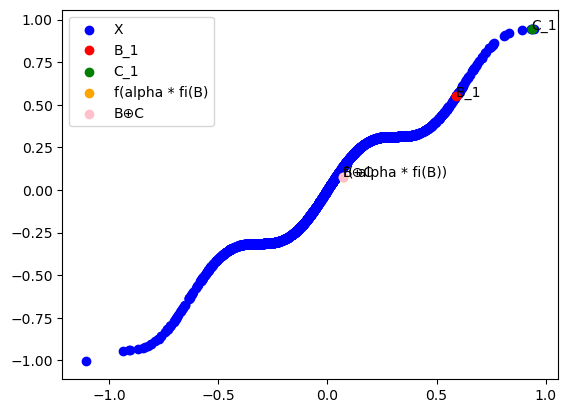
\includegraphics[width=0.9\linewidth]{./images/alpha1.png}
                        \end{column}
                        \begin{column}{0.5\textwidth}
                            \centering
                            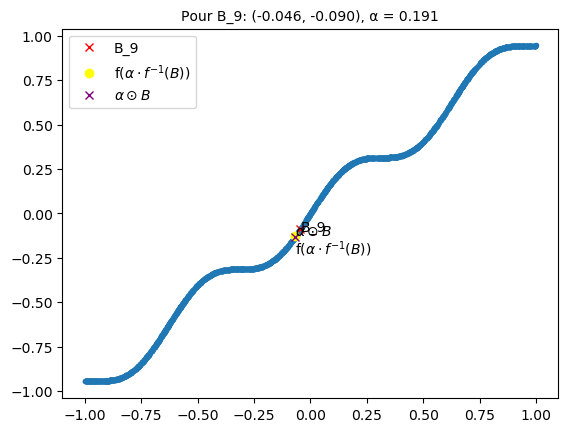
\includegraphics[width=0.9\linewidth]{./images/alpha4.png}
                        \end{column}
                    \end{columns}
                \end{frame}
                %---------------------------------------------------------------------------------
                \begin{frame}
                    As conclusion, we see that the error between the Direct Sum and the morphism of the sum of the inverse morphism is to ordre 3, and the error between the scalar multiplication and the morphism of the scalar multiplication of the inverse morphism is also to ordre 3 . This means that the model is effectively learning the properties of the vector space and accurately reproducing the binary operations defined on the dataset.\\
                    So we conclude that $(V,\oplus,\odot)$ is a vector space with an algebraic structure
                    
                \end{frame}

                \section{Conclusion}
                \begin{frame}
                    \frametitle{Conclusion}
                    The project provides a comprehensive 
                    exploration of algebraic structures and
                    their relevance in data analysis, 
    offering insights into how these 
    structures can be effectively applied 
    to detect patterns and derive meaningful
    conclusions from datasets. Through Python 
    implementation and testing, the project 
    demonstrates practical approaches to 
    optimize algebraic structures for 
    improved accuracy and performance 
    in various applications. However, there is still a 
    challenge to continue working to generalize the latter to 
    differential equation, as we discussed in the introduction.
    \end{frame}

    \section{References}
    \begin{frame}
        \frametitle{References}
        \begin{itemize}
            \item \url{https://en.wikipedia.org/wiki/Algebraic_structure}
            \item \url{https://pytorch.org/docs/stable/torch.html}
            \item Thomas A. Farmer, Article : The College Mathematics Journal, Miami University, Oxford, OH 45056-1602, USA. 
            
        \end{itemize}
    \end{frame}



    \begin{frame}
        \centering
        \Huge{Thank you for your attention !}
    \end{frame}




\end{document} 

